\subsection{Experiment Setup} \label{Experiment_Setup}

The experiment consists of AAC six sampling bags subsystem, and the CAC coiled tube subsystem. The principal aim is to validate the AAC sampling method and to do so, it is necessary to sample during descent phase in order to compare the results with the ones obtained from the CAC. All speeds mentioned in this section have been obtained from the BEXUS manual as well as through analysis of past flights.

The primary concern regarding the AAC air sampling subsystem is that after cut-off the gondola will tumble and fall at an average speed of 50 m/s for approximately 2 minutes \cite{BexusManual}. This falling speed is too fast in order to sample air at the desired vertical resolution that is targeted to be 500m. This means that only after the gondola is stabilized at a descent rate of 8 m/s \cite{BexusManual} the sampling can be done. The tumbling phase will span approximately for 6km and considering a floating phase at 25km, the sampling can be started from 19km in altitude. Nevertheless, the main region of interest is the stratosphere, especially between 19km and 25km of altitude. It is for this reason that the team has decided to sample during ascent phase as well. Six sampling bags will be filled up, two during ascent phase approximately between 18-22km, and four during descent phase below 18km. The desired vertical resolution is 500 m at a falling speed of 8 m/s which means that using bags with a volume of 3L, an air pump with at least 3L/min intake rate is necessary for the sampling bags.

The maximum pressure that the sampling bags can withstand has to be taken into account in order to avoid bursting. During ascent phase, due to the decreasing pressure, the bags with the air samples , will expand which may have risk of bursting. To avoid this, the bags should not be fully sampled. The providers recommend not to fill more than 80\% (~2psi/0.14bar) for Multi-Layer Foil bags. The opposite applies for descent phase. The bags with the air samples, will be compressed, and in order to assure that the samples are enough for analysis, they should be fully filled. It has to be mentioned that it has been found from past research \cite{LISA} that the same bags can withstand a difference in pressure between outside and inside of 310hPa at 30km of altitude, which is equivalent to 0.31bar. Therefore, future test will confirm the maximum pressure for the bags.

Depending on the altitude of sampling, the range of the sample size is between 0.2L and 0.8L, with 0.2L being the minimum amount required for the chromatographer to analyze. 

The AAC will need an air pump for sampling, due to low ambient pressure at stratospheric altitudes. The air pump is also needed in order to assure the intake flow rate and obtain a good resolution. A control valve will be used to flush the AAC system after each bag is filled and make sure that the next bag will be filled with fresh air from the corresponding altitude. Each sampling bag will be assigned a 500 meter altitude sampling range from which to collect air samples. At an ascent speed of 5 m/s during the Ascent Phase and at a descent speed of 8 m/s during the Descent Phase. 

Shortly after the launch, the CAC valve will be opened in order to allow flushing the fill gas that is inside the tube, while the AAC valves will be closed until reaching the sampling altitude. Flushing of the CAC tube happens passively through the progressive decrease in air pressure during the balloon's ascent phase. The CAC valve will remain open at all time during ascent, floating, and descent phases. The tube will empty itself due to pressure gradient during the ascent phase and it will be filled passively during descent. The valve will close just after hitting the ground in order to preserve the sample. 
%The AAC will need an air pump for sampling, due to low ambient pressure. The air pump is also needed in order to assure the intake flow rate and obtain a good resolution.

%After sampling for a given bag is complete, the pump will be flushed and prior to the subsequent sampling bag valve being opened. This process continues until the last sampling bag is filled.
This procedure occurs twice, the first time during the Ascent Phase for the 2 first sampling bags and the second time during the descent phase for the remaining 4 sampling bags.

The ambient pressure will be measured by three pressure sensors located inside the experiment box. Only one of them is necessary for AAC and CAC, but using three will provide redundancy. The pressure inside the AirCore is assumed to be the same as the ambient pressure, therefore no sensor is needed. To measure the pressure inside the bags, three more sensors will be allocated inside the valve center. To measure the ambient temperature in the AirCore, three sensors will be allocated in the AirCoil box (in the styrofoam). Temperature inside the AirCore is assumed to quickly adjust to the ambient temperature, therefore there will not be differentiation in between inside/outside temperature. For the bags three more temperature sensors will be placed in the bags' box (in the styrofoam). To control the temperature in the electronics box, valve center and the pump box, one temperature sensor will be used in each of them. In total, there will be six pressure sensors and nine temperature sensors. 


The sampling of the AAC will be triggered by the pressure reading from the sensors inside the valve center. When the required pressure is reached, the valve will open and the sampling will start. The closing of the valve depends on two conditions and it will be triggered when either one of the conditions is true. These conditions are: maximum sampling time or maximum pressure difference between inside/outside the bags. They are determined from past research but in the future will be determined by testing. 

The emptying and sampling sequence is represented in Figures \ref{fig:ascent} and \ref{fig:descent}. It should be kept in mind that the different pressures are what triggers the opening of the valves. 

\begin{figure}[H]
    \begin{align*}
        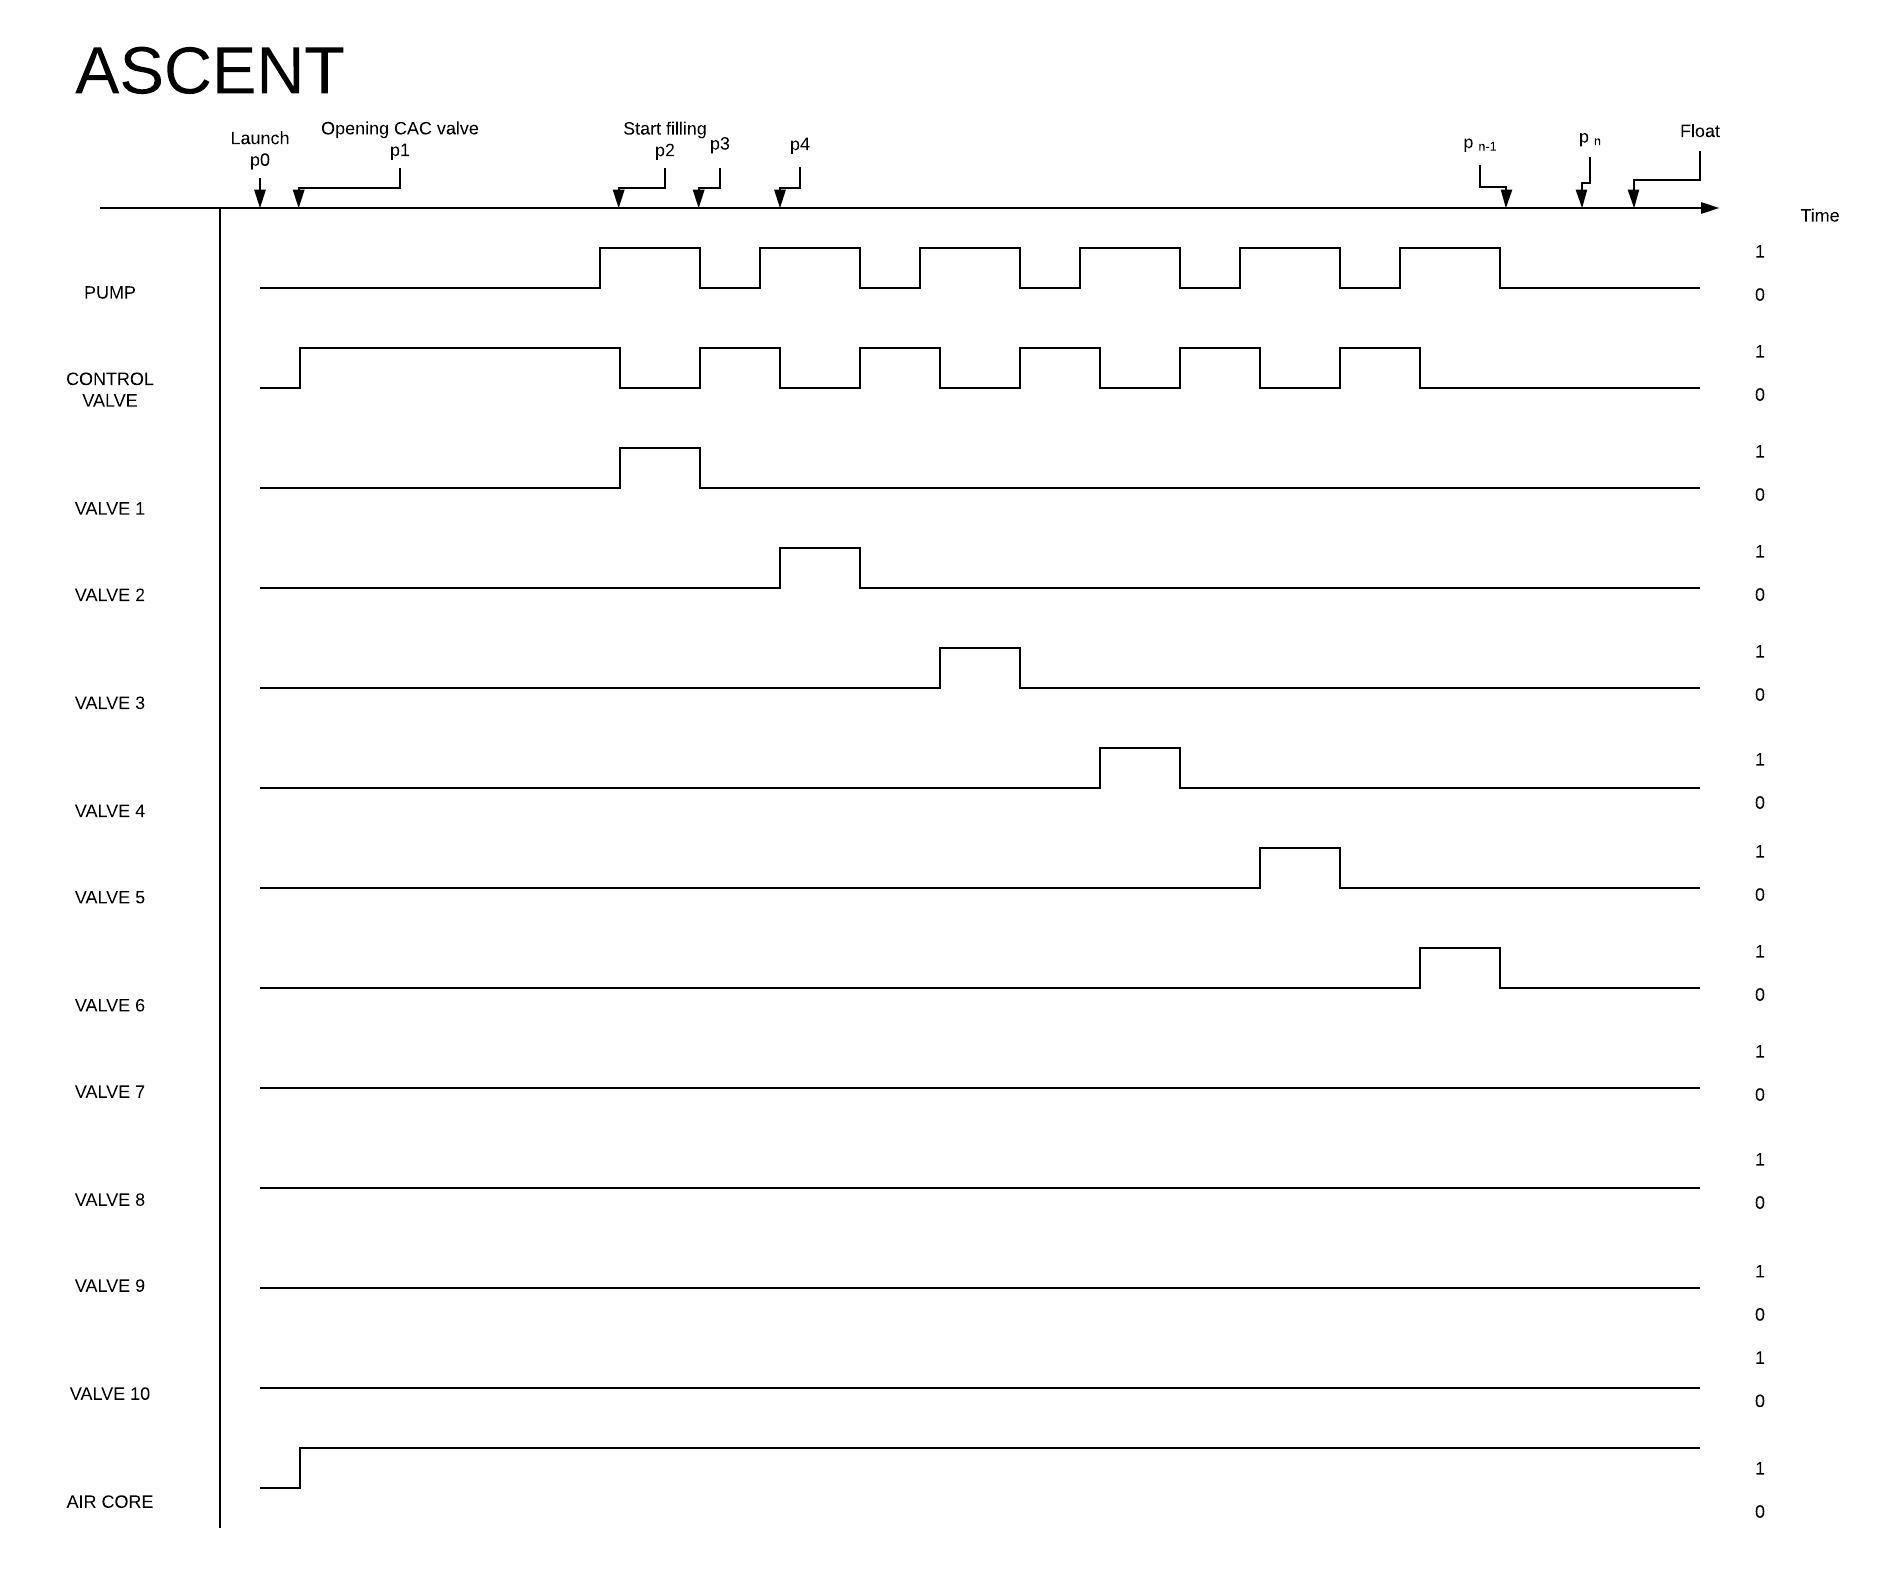
\includegraphics[width=1\linewidth]{4-experiment-design/img/ascent-phase.jpeg}
    \end{align*}
    \caption{The emptying and sampling sequence-Ascent Phase\label{fig:ascent}}
\end{figure}

\begin{figure}[H]
    \begin{align*}
        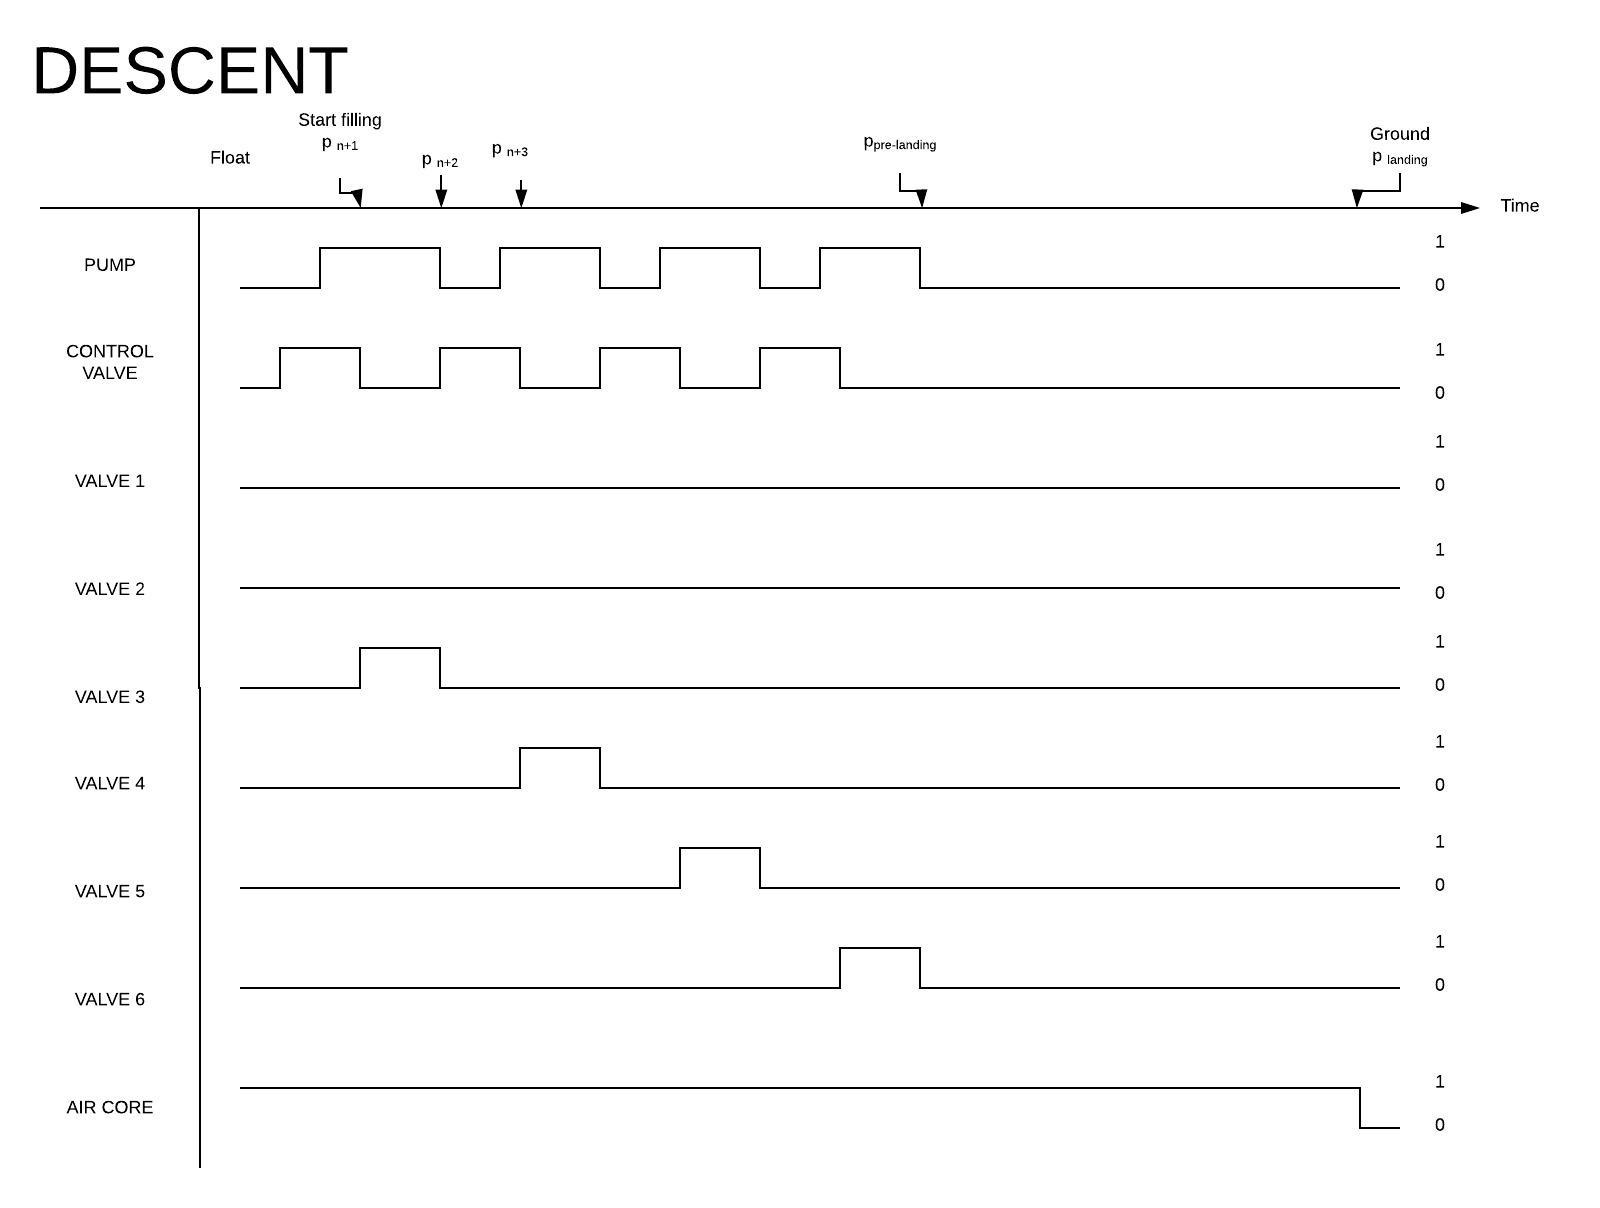
\includegraphics[width=1\linewidth]{4-experiment-design/img/descent-phase.jpeg}
    \end{align*}
    \caption{The emptying and sampling sequence-Descent Phase\label{fig:descent}}
\end{figure}

In the diagrams, 0 denotes closed/off and 1 denotes opened/on.

The general timeline of the experiment is as follow:

\textbf{Ascent Phase:}\\
$p_0$ – $p_1$
\begin{itemize}
    \item CAC valve shall be closed.
    \item AAC valves shall be closed.
    \item AAC' control valve shall be closed.
    \end{itemize}
$p_1$ – $p_2$
\begin{itemize}
    \item CAC valve shall be opened.
    \item AAC valves shall be closed.
    \item CAC tube shall be flushed.
    \item AAC' control valve shall be open.
    \end{itemize}
$p_2$ – $p_3$
\begin{itemize}
    \item Sampling bags' control valve shall be closed.
    \item Sampling bag valve 1 shall be opened, allowing for air to enter the first bag.
    \item CAC valve remains open.
    \end{itemize}
$p_3$ – $p_4$
\begin{itemize}
    \item Sampling bag valve 1 shall be closed
    \item Sampling bags' control valve shall be opened, allowing the system to flush. 
    \end{itemize}
$p_4$ - $p_n$
\begin{itemize}
    \item The above procedure shall repeat itself until the remaining one bag has collected air sample for its assigned altitude.
    \end{itemize}



\textbf{\\Float Phase:}\\
No action taken other than continued telemetry.
\begin{itemize}
    \item Sampling bag valve 2 shall be closed.
    \item Sampling bags' control valve shall be closed.
    \item Air pump is off.
\end{itemize}
 
\textbf{Descent Phase:}

Note: Before sampling starts again, the system has to be flushed. 

$p_{n+1}$ – $p_{n+2}$
\begin{itemize}
    \item Sampling bags' control valve shall be closed.
    \item Sampling bag valve 3 shall be opened, allowing for air to enter the first bag.
\end{itemize}

$p_{n+2}$ – $p_{n+3}$
\begin{itemize}
    \item Sampling bag valve 3 shall be closed
    \item Sampling bags' control valve shall be opened, allowing the system to flush. 
\end{itemize}

In between, same procedure shall repeat itself until all the remaining bags have collected air samples for their assigned altitudes.

$p_{pre-landing}$ 
\begin{itemize}
    \item System Sampling bag valve 6 shall be closed.
    \item Sampling bags' control valve shall be closed
    \item CAC valve shall be opened.
\end{itemize}


$p_{landing}$
\begin{itemize}
    \item CAC valve shall be closed.
\end{itemize}


Note: The AAC system's air pump is only on during sampling into the air sampling bags and flushing of the system.


\raggedbottom